\chapter{Compute Unified Device Architecture - CUDA }\label{chap:CUDA}
\section{Introduction}
\begin{wrapfigure}{I}{0.45\textwidth}

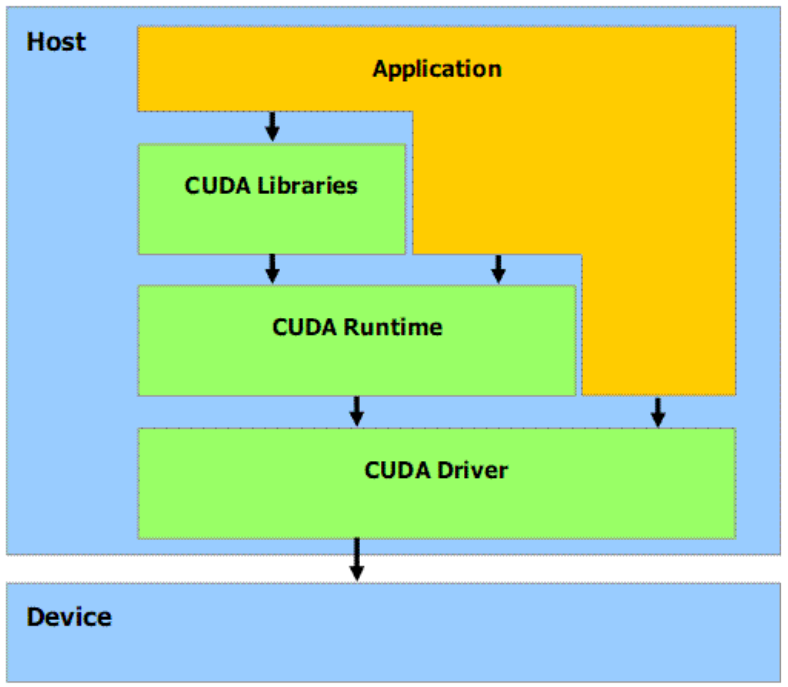
\includegraphics[scale=0.23]{./images/cudaArchitecture}
\caption{Cuda Software Stack}\label{CUDA_SOFT_ARCH}
\end{wrapfigure}
In November 2006 Nvidia released CUDA a platform (both hardware and software)
that allow the developers to use an high-level programming language
(e.g. C with slightly additions) to exploit the parallel power of the
hardware in order to solve complex computational problems in a more efficient
way than on a CPU. CUDA is attractive because is a complete system(software and
hardware model map well onto each other aiding the developer comprehension),
from silicon to high-level libraries and a growing experience exists providing a valuable resource to developers.
It is for these reason CUDA was selected as development platform for this work
rather than other platforms\footnote{e.g. OpenACC that proved to be
unsuitable to the parallelization of SCIARA-fv3}.
CUDA expose three level of components to an application (See figure
\ref{CUDA_SOFT_ARCH}):
\begin{enumerate}
\item \textit{\textbf{Cuda Driver}}:
	\begin{itemize}
	  \item Distinct from graphics driver. The only purpose of this component is to
	  provide the access to the GPU's general purpose functionalities.
	\end{itemize}
\item \textit{\textbf{CUDA Runtime}}:
	\begin{itemize}
	  \item Built on top of the CUDA Driver, provide an higher level of
	  abstraction making the code less cumbersome  especially as far as the
	  complexity of host code for kernel launches is concerned. 
	\end{itemize}
\item \textit{\textbf{CUDA Libraries}}:
 \begin{itemize}
	  \item Built on top of the CUDA Runtime, Is a collection of Libraries(CUBLAS,
	  CUSP, CUFFT, Thrust etc.)\footnote{For example CUFFT
	  provides an interface for computing Fast Fourier Transform
	  up to 10x faster than CPU
	  (\url{https://developer.nvidia.com/gpu-accelerated-libraries}).} providing full-suitable state of the art implementation of algorithms for a wide range of applications.
	\end{itemize}
\end{enumerate}


\FloatBarrier


\section{CUDA Hardware model}
There are various kind of CUDA capable device on the market. From a mid-level
laptop graphic card to a numerical computation dedicated
card.\footnote{For example GeForce GT 620M and Kepler K20x are respectively a
laptop and a dedicated numerical computation CUDA capable device.}
The Nvidia GPU hardware architecture is built around a scalable array of multithreaded \emph{Streaming Multiprocessors (SMs)}.
The \emph{Streaming Multiprocessors} is designed to execute hundreds of threads
concurrently  and contains a number of Streaming Processors (SP)\footnote{The SP
cores are also called \emph{CUDA cores} and the number of them depends on the
compute capability (See section \ref{computeCapability}) of the device. For
example v3.5 CUDA capability GPUs SM consists of 192 SPs. For v2.1
this number is 48, and for the old v1.x it is 8.}.





\subsection{Compute Capability}\label{computeCapability}
Each device comes with a revision number which defines the \emph{compute
capability} of the device, and it determines the set of features that can be
used for programming and the configuration in processors and memory.
The compute capability of a device is defined by a major revision number and a
minor revision number. Devices with the same major revision number are of the
same core architecture. The major revision number is 3 for devices based on the Kepler architecture, 
2 for devices based on the Fermi architecture, and 1 for devices based on the Tesla architecture.
The minor revision number corresponds to an incremental improvement to the core
architecture, possibly including new features\footnote{Here the table full
specification and features per Compute Capability:
\url{http://docs.nvidia.com/cuda/cuda-c-programming-guide/index.html\#compute-capabilities}}.
Furthermore, properties and features support can be queried using the runtime
API.
 Accelerators with capability 3.5, for example, were enhanced by dynamic
 parallelism(See section \ref{DynamicParallelism}).
 
 For this work we used as hardware test the Nvidia GeForce GTX 780 a GeForce GTX
680  respectively with compute capability 3.0 and 3.5 Kepler architecture and a
GeForce GTX 480 and GeForce GTX 580 both compute capability 2.0, Fermi
architecture.
For brevity purpose we are going to see in detail just the new Kepler
architecture.
\FloatBarrier
\subsection{Kepler Architecture}\label{sect:keplerArch}

NVIDIA Kepler architecture builds on the foundation first established in 2010 with NVIDIA's Fermi GPU
architecture.
The first GPU based on this new Kepler architecture, code-named ``GK104'' is
fabricated on a 28nm process, and every internal unit was designed for the best perf/watt possible. The
first product being introduced based on GK104 is the GeForce GTX 680.
Like Fermi, Kepler GPUs are composed of different configurations of Graphics
Processing Clusters (GPCs), Streaming Multiprocessors (SMs), and memory controllers.
The GeForce GTX 680 GPU consists of four GPCs, eight next-generation Streaming
Multiprocessors (SMX), and four memory controllers. In GeForce GTX 680, 
each GPC has a dedicated raster engine and two SMX units. With a total of eight
SMX units, the GeForce GTX 680 implementation has 1536 CUDA Cores (See figure
\ref{gtxArch} and table \ref{tab:cudaGtxspec}).
\begin{figure}
\centering
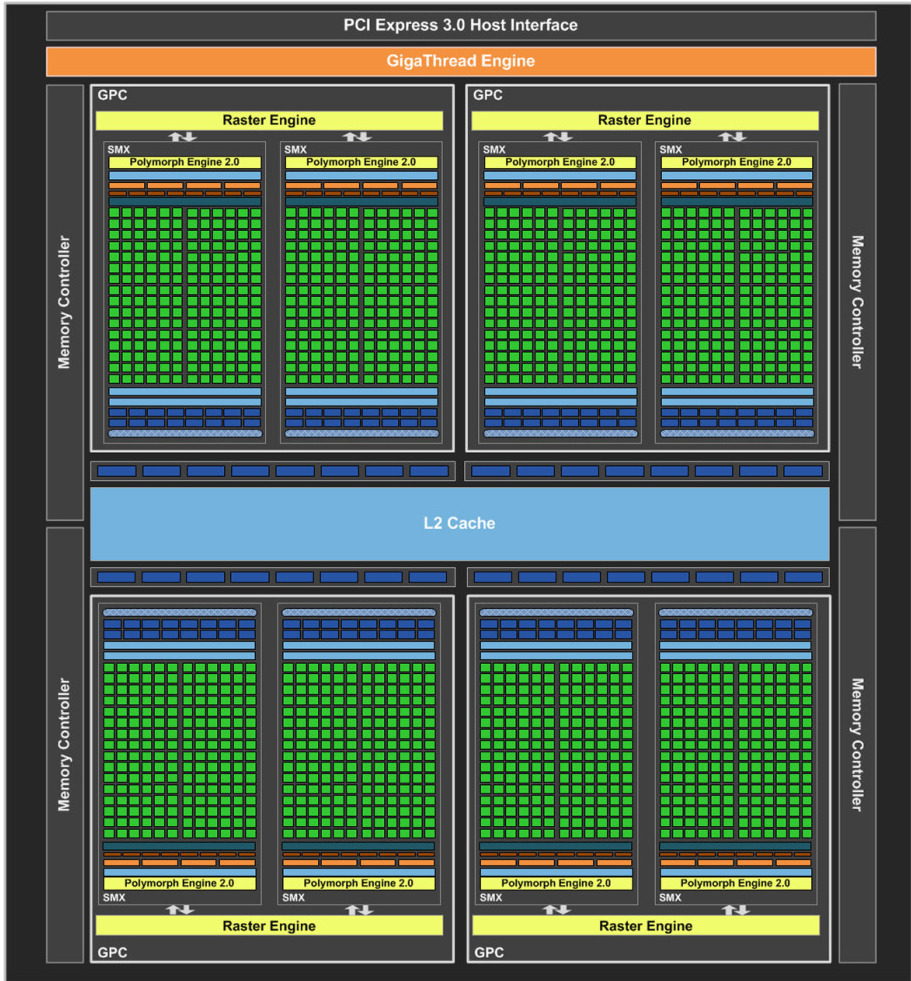
\includegraphics[scale=0.5]{./images/gtxArch}
\caption{Kepler Architecture (GTX 680)}\label{gtxArch}
\end{figure}
\FloatBarrier
Tied to each memory controller are 128KB L2. 
With four memory controllers, a full GeForce GTX 680 GPU has 512KB
L2 cache.

\begin{table}
	\centering
    \caption{High-level comparison of Kepler vs. Fermi GPUs}
\label{tab:cudaGtxspec}
\begin{tabular}{ | l | l | l |}
    \hline
    \textbf{\textit{GPU}} 		& \textbf{\textit{GTX 680}} &
    \textbf{\textit{GF110(Fermi)}}
    \\ \hline \textbf{\textit{Transistor}}  & 3.54 billion & 3.0    billion\\
    \hline \textbf{\textit{CUDA Cores}}  & 1536		  & 512\\ \hline
    \textbf{\textit{Graphic Core Clock}}  & 772 MHz & 1006 MHz  \\ \hline
    \textbf{\textit{GFLOPs}}  & 3090 & 1581\\ \hline
    \textbf{\textit{Memory Clock}}  & 6008 MHz & 4008 MHz\\ \hline
    \textbf{\textit{Memory Bandwidth}}  & 192.26 GB/sec & 192.4 GB/sec\\ \hline
    \textbf{\textit{TDP}}  & 195 W & 244 W\\ \hline
\end{tabular}   
\end{table}
    

\subsubsection{Streaming MultiProcessor-SMX}
The SM is the heart of NVIDIA unified GPU architecture. Most of the key
hardware units for graphics processing reside in the SM. The SM CUDA cores perform pixel/vertex/geometry shading and
physics/compute calculations. Texture units perform texture filtering and load/store units fetch and
save data to memory. Special Function Units (SFUs) handle transcendental and graphics interpolation
instructions. There are eight SMX in GeForce GTX 680 instead of sixteen as in
the GTX580).
\begin{wrapfigure}{r}{0.45\textwidth}
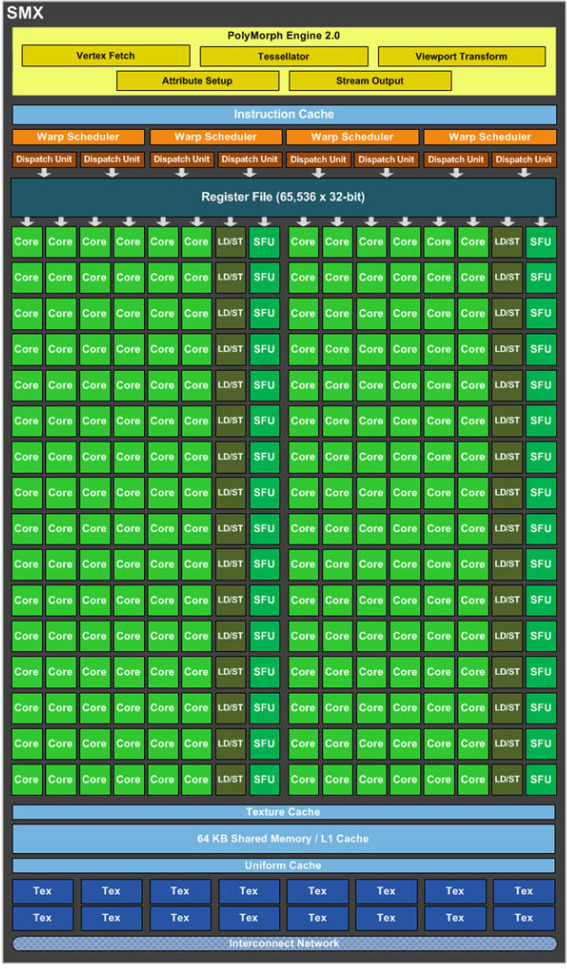
\includegraphics[scale=0.5]{./images/gtx680_SMX}
\caption{GTX 680 SMX Architecture Detail}\label{gtx680_SMX}
\end{wrapfigure}
To feed the execution resources of SMX, each unit contains four warp schedulers, and each warp
scheduler is capable of dispatching two instructions per warp every clock.
More importantly, the scheduling functions have been redesigned with a focus on power efficiency. For
example: Both Kepler and Fermi schedulers contain similar hardware units to handle scheduling
functions, including, (a) register score boarding for long latency operations (texture and load), (b) inter-
warp scheduling decisions (e.g., pick the best warp to go next among eligible candidates), and (c) thread
block level scheduling (e.g., the GigaThread engine);
The SMX schedules threads in groups of 32 parallel threads called warps. Each SMX features four warp 
schedulers and eight instruction dispatch units, allowing four warps to be issued and executed 
concurrently. Kepler's quad warp scheduler selects four warps, and two
independent instructions per warp can be dispatched each cycle. 
All cores in a multiprocessor have on-chip shared resources, including 255 local
32- bit registers per thread and one on-chip fast memory of size 64Kbyte, which
enable threads cooperation and transparent caching\footnote{it is possible to
use as user managed cache max of 48kb. There are two shared memory configuration
available per kernel. 16kb cache and 48kb user managed or viceversa.}.
Threads variables typically reside in live registers. The on-chip shared memory has
very low access latency and high bandwidth similar to an L1 cache; it holds CUDA variables
for the active thread blocks. The shared memory allows the parallel threads run on the cores in
a MP to share data without sending it over the system memory bus.




\FloatBarrier
\newpage
\section{CUDA Programming model}\label{cudaProgrammingModel}

CUDA programming model is designed to fully expose parallel capabilities of NVIDIA GPUs.
Even though the language is devoted to general purpose computing, it still requires the
programmer to follow a set of paradigms arising from the GPU architecture.
CUDA provides a few easily understood abstractions that allow the programmer to
focus on algorithmic efficiency and develop scalable parallel applications by expressing the
parallelism explicitly. It provides three key abstractions as hierarchy of
thread groups, shared memories, and synchronization barrier that provide a
clear parallel structure to conventional C code for one thread of the hierarchy.
\begin{wrapfigure}{l}{0.55\textwidth}
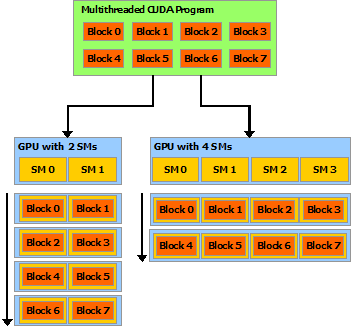
\includegraphics[scale=0.9]{./images/automatic-scalability}
\caption{Automatic Scalability}\label{automatic-scalability}
\end{wrapfigure}
\FloatBarrier
The abstractions guide the programmer to partition the
problem into coarse sub-problems that can be solved independently in parallel, and then into
finer pieces that can be solved cooperatively in parallel. The programming model scales
transparently to large numbers of processor cores: a compiled CUDA program executes on any
number of processors, and only the runtime system needs to know the physical
processor count (See figure \ref{automatic-scalability}).

\subsection{Host and Device}
CUDA paradigm is heterogeneous computation:
serial portions of applications are run on the CPU, and parallel portions are
off loaded to the GPU.
The CPU and GPU are treated as separate devices that both host and device
are equipped with their own memory spaces(referring to them, respectively as to
the host memory and device memory). This configuration also allows simultaneous and overlapped

\subsection{Kernels Functions And Thread Hierarchy}\label{kernels}
\begin{wrapfigure}{l}{0.540\textwidth}
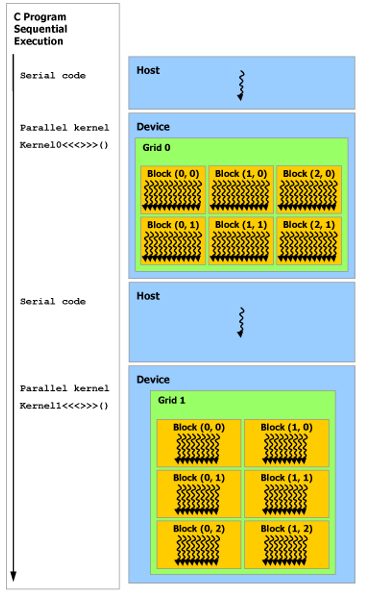
\includegraphics[scale=0.9]{./images/heterogeneous-programming}
\caption{Heterogeneous Programming}\label{heterogeneous-programming}
\end{wrapfigure}
Host code schedules kernels to be executed on the GPU, which also specifies
starting configuration of the kernel.
Kernel code is compiled by nvcc the Nvidia CUDA compiler and sequential code by
the host's normal C\footnote{For example GCC on Unix or Visual C++ on Windows
systems.} compiler which is then linked to create a single binary executable.
A kernel can be ``launched'' using thousands
or even millions of “lightweight� threads that are to be run on the device.
computation on both the CPU and GPU without contention for memory resources (See figure \ref{heterogeneous-programming}).
The programmer is encouraged to “think big� and schedule threads liberally and
as needed. Cuda threads are thought as lightweighted for these because there
is not any creation overhead and can be created quickly, scheduling of blocks
and threads is handled directly on hardware avoiding any software overhead. 
More threads can hide latency caused by data fetching, leading to performance gains.
A kernel is an extension to the standard C function that are executed N times
by different N threads(as opposed to only one like regular C function).
 kernel is defined specifying the \textbf{\color{green} \_\_global\_\_} keyword
and the \textit{execution configuration}
\textless\textless\textless \ldots \textgreater\textgreater\textgreater. Each
thread is given a unique \textit{threadID} that is accessible through the
built-in variable(a 3-component C-structure) threadIdx. (See listing
\ref{code:kernelInvocation} at page \pageref{code:kernelInvocation}).

The threads are organized by the programmer by defining a grid and making a division
of the grid in thread blocks or just blocks, (see figure \ref{threadHierarchy}
and \ref{kernelGrid}).
The index of the blocks and threads in x, y and z direction can be retrieved
,within a kernel, via statements like: by = blockIdx.y, and tz = threadIdx.z (as
well as the grid dimension via dimGrid.(x,y,z)).
We can assign a unique (for the grid) global ID to each thread by combining
both thread and block index, e.g. for a 2D grid and 2D block \(threadIDx = blockDim.x
\times blockIdx.x + threadIdx.x \) and \(threadIDy = blockDim.y \times blockIdx.y +
threadIdx.y\). It is useful when we want to assign a portion of work to each
thread and divide the work among them\footnote{E.g. In a parallel matrix
summation algorithm we can assign a unique pair of matrix's cells to be summed
to each thread, and them could retrieve the correct pair just using their global
ID.}
\begin{center}
\begin{figure}
\centering
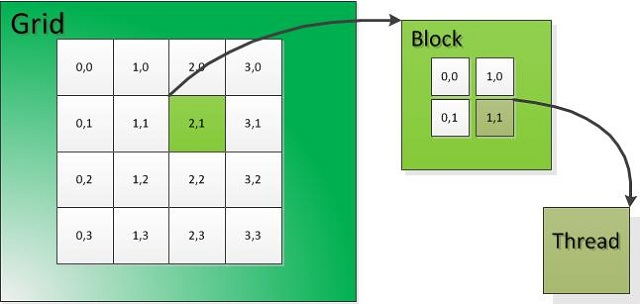
\includegraphics[scale=0.8]{./images/thread_hierarchy1}
\caption{The CUDA architecture on a conceptual level. The grid is divided into blocks that each consists of a number
of threads.}
\label{threadHierarchy}
\end{figure}
\end{center}
\FloatBarrier

Each block consists of a batch of threads, and can be a 1D, 2D or 3D object.
This provide a natural and intuitive way to compute on data structure like
array(1D), matrix(2D) or volume(3D).
\begin{figure}
\centering
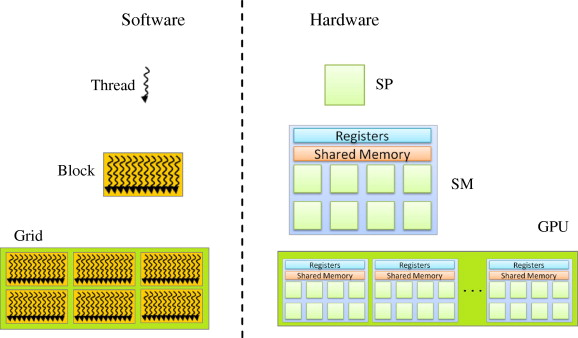
\includegraphics[scale=1.1]{./images/mappingSofthard}
\caption{Mapping Hardware-Software}\label{mappingSofthard}
\end{figure}

\begin{wrapfigure}{r}{0.62\textwidth}
\caption{Kernels Grid}\label{kernelGrid}
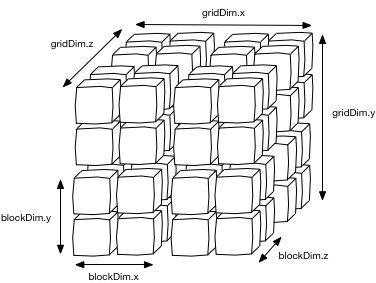
\includegraphics[scale=0.66]{./images/cuda-grid}
\end{wrapfigure}
The maximal number of threads per block and
the maximum dimensionality of the grid and the block which is allowed depends on
the compute capability (section \ref{computeCapability})and that limit exist because all threads of a
block reside on the same multiprocessor and they share its resources as
shared/registers memory or cores. On GTX 680 the maximum number of thread per
block is 1024 and the maximum sizes of each dimension of a block is \begin{math}1024 \times 1024 \times 64\end{math}.

It means that, the dimensionally of a
block launched on a GTX 680 must satisfy:
\[
\begin{cases} 

			xBlockDim \times yBlockDim \times zBlockDim=1024 \\
			 1\le xBlockDim \le 1024 \\
			  1\le yBlockDim \le 1024 \\
			  1\le zBlockDim \le 64\\  
\end{cases}
\]
Plus a kernel can be launched and executed only by equally shaped kernel so the
total number of threads is the number of threads per block times the number of blocks\footnote{Blocks of
\(32\times32\) threads are allowed as well as \(16\times16\times2\). Blocks of
\(2\times2\times128=512\) threads are not allowed because zDim is greater than zDim's limit(64).
\(16\times16\times16=4096\) is not allowed because 4096 is greater than the maximum
permitted number of thread per block.}.
The blocks are divided amongst the physical processors of the GPU, and threads
inside a block are grouped in warps.
A warp consist typically of 32 threads with consecutive indices that are in
principle having their instructions executed simultaneously on the
multiprocessor\footnote{The scheduler(one or more per SM) select threads for
execution in granularity of warps. Hence the name of \emph{warp
scheduler}.}(SIMD).
If one or several threads executes conditional code that differ in code path
from other threads in the warp (SIMT), these different execution paths are
effectively serialized, as the threads need to wait for each other. This
phenomenon is referred to as \emph{thread divergence}\label{threadDivergence}
\footnote{A common situation that cause divergence involves branch condition
that are function of the thread id and the branch granularity is not a whole
multiple of the warp size, and so not all the threads in the same warp follow the same path.
E.g.: \(if (threadIdx.x \ge 5)\) is divergent code instead of 
\(if (threadIdx.x / WARP\_SIZE > 2)\) that avoid divergence unless it has a
branch condition dependent on thread id.
}, a situation that should be avoided as much as possible.
Threads inside a block can cooperate by communicating and sharing (see section
\ref{shareMemory}) data through shared memory or by synchronizing their
execution via the \textbf{\_\_syncthreads()} intrinsic function that acts as barrier at block
level. 

\subsection{Memory model}\label{memoryModel}


Different kind of memories can be accessed by threads during their execution,
and can be classified regarding their degree of privacy and their speed (See
table \ref{tab:memoryHierarchyScope}).
All threads have free access to \emph{global memory} or also called \emph{device
memory}. Threads within the same block have access to so called \emph{shared
memory} that can be used for cooperation between thread of the same block and,
at the end, each thread has his own local and private \emph{registers}. There
are other two memory spaces that can be addressed by all threads: constant and
texture memories each specialized for different usage, but the shared
characteristic is that they are persistent across kernels launch\footnote{Within
the same application.}.



\subsubsection{Device Memory}
\begin{wrapfigure}{r}{0.5\textwidth}
\caption{Memory Hierarchy}\label{memoryHierarchy}
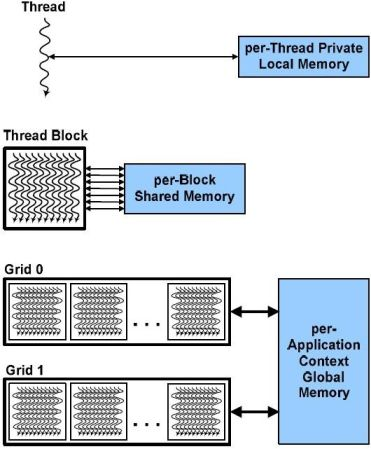
\includegraphics[scale=0.9]{./images/memoryhierarchy}
\end{wrapfigure}

The most prominent feature of device memory is its high capacity,
up to 6GB (Tesla C2070), but is also slow (400 - 600 cycles
latency)\footnote{New devices are equipped with L2 cache (in Kepler 1.5MB), that
helps to mitigate this problem serving either load and write operations.}
prohibiting an extensive usage, when high performance is requested.
Parts of the DRAM are dedicated to constant memory and texture memory.

\subsubsection{Global Memory}
The most general space allowing both, reading and writing of data, is
the global memory. It is allocated and is allocated and managed 
by the host. Due to DRAM bandwidth optimizations and the GPU architecture, and, 
as each multiprocessor works independently, unordered reads and writes are
possible because all threads are able to read from all memory spaces at any
time without any mutual exclusivity mechanism. Is up to the programmer to avoid
race-conditions and incoherences.

An important concept related to the global memory that has to be kept in mind
when writing CUDA C code due to its performance consequence, it's the
memory coalescence.

 \hfill \\ \hfill \\
 \begin{table}
\caption{Memory architecture summary.}
 \label{tab:memoryHierarchyScope}
\begin{tabular}[l]{|l|l|l|l|l|l|}
\hline 
\textbf{Memory} & \textbf{Location}&  \textbf{Chached}& \textbf{Access} &
\textbf{Scope} & \textbf{LifeTime}\\ \hline \hline

\textit{Register} & On-Chip	 & N\textbackslash A	& R\textbackslash W & One
Thread & Thread\\
\hline \textit{Local} & Off-Chip & NO	& R\textbackslash W & One Thread & 
Thread\\ \hline \textit{Shared} & On-Chip  & N\textbackslash A & R\textbackslash W & All
Threads in a block & Block\\
\hline \textit{Global} & Off-Chip & NO 	& R\textbackslash W & All Threads +
Host & Application	\\
\hline \textit{Constant} & Off-Chip & YES  & R & All Threads + Host & 
Application\\
\hline \textit{Texture} & Off-Chip & YES  & R & All Threads + Host &
Application \\
\hline
\end{tabular}
\end{table}
\subsubsection{Coalescence}
Coalescence is the capability of the device of grouping global memory accesses
of threads whithin a warp.
Global memory loads and stores by threads of a warp \footnote{Half warp for
devices of compute capability 1.x)} are coalesced by the device into as few as
one transaction when certain access requirements are met.
Remanding that c.c. 3.5 global memory is only L2 cached, while for devices with
c.c. 2.x the concurrent accesses of the threads of a warp will coalesce into a
number of transactions equal to the number of cache lines necessary to service
all of the threads of the warp. By default, all accesses are cached through L1,
which has 128-byte lines. For scattered access patterns, to reduce overfetch, it
can sometimes be useful to cache only in L2, which caches shorter 32-byte
segments

In order to achieve coalescence there should be some
coherence\footnote{Depending on Compute capability, access requirements are
different and usually less constrained with newer devices.} in memory access by
adjacent threads running on the device.
Certain memory access patterns enable the hardware to coalesce groups of reads
or writes of multiple data items into one operation. Data that cannot be laid
out so as to enable coalescing (in general case) and, application that do not
exploit this feature will tend to see lesser speedups when used in computations
on CUDA.
Assuming compute capability 2.x the very first pattern that enable coalescence
is when the \(k-th\) accesses the \(k-th\) word in a cache line\footnote{128B
aligned memory} (not all threads need to partecipate).
Morever if the same scenario of sequential access happens, but on misaligned
with the cache line, two 128B loads are required in order to fill the L1 cache
or even more if L2 is used (see figure \ref{fig:misaligedCoalescence}, in red
loaded memory portions).
\begin{figure}
\centering
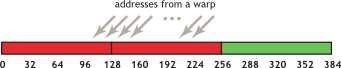
\includegraphics[scale=1.0]{./images/unaligned-sequential-addresses}
\caption{Parent Child Synchronization.}\label{fig:misaligedCoalescence}
\end{figure}


 
\subsubsection{Texture Memory}
As its name suggests, texture memory is used for storing textures.
Although this memory was designed for the classical openGL and DirectX graphic
pipeline (see section \ref{graphicPipeline}) it can be used successfully in some scenario to
accelerate the application especially when the memory access pattern exhibit
2D-spatial \footnote{A texture has
2-dimensions, so it's not surprising if this kind of memory is optimized
for 2D accesses.} locality it will give higher memory bandwidth by reducing requests to
the off-chip DRAM. Threads of the same warp that read texture addresses that are
close together, will achieve better performance using the texture
cache\cite{NvidiaprogGuide}. 

\subsubsection{Constant Memory}\label{sect:constantmemory}
Specific part of device memory is the constant memory, which allows to store limited
amount (64KB) of constant symbols. Similarly to the texture memory, the accesses
are cached but only reading is allowed. Constant memory should be used for small
variables that are shared among all threads and do no require interpolation.
It is declared by the host using the keyword \textbf{\_\_constant\_\_}, and its
size is to be known at compile time. There are two main reason why reading from
constant memory can save bandwidth:

\begin{itemize}\itemsep1pt
  \item A single read can be broadcasted to all thread of the same \emph{warp}.
  \item Constant memory is cached, so consecutive reads of the same address will
  not incur any additional traffic on off-chip DRAM.
\end{itemize}

\subsubsection{Shared Memory}\label{shareMemory}
Present on each SM. On the Fermi architecture card, there is 64KB of level 1
cache made up of SRAM. SRAM, or static random-access memory, is an expensive type of RAM, that
is much faster than DRAM. This cache is divided into two parts: a normal cache and a user managed
cache called the shared memory\cite{NvidiaprogGuide}. Depending on the program,
the L1 cache can be set to either be 16 or 48 KB, where the size of shared memory is the remainder.
As programmer the keyword \textbf{\_\_constant\_\_} make a variable resident
into shared memory. Cuda will create a copy of each variable for each block.
Each thread within a block share the \emph{shared memory}, and so, can modify or
read whichever address, but it cannot access to any other block's copy.
This provide an excellent mechanism by which threads can communicate and cooperate
on computations. It is a on-chip SRAM\footnote{Static random-access memory, more
expensive and less dense than DRAM.} and is very fast compared to the \emph{global
memory} (30-50 cycles latency) but it is only alive during the kernel call.
More in detail, shared memory is divided into multiple banks\footnote{That
number is fixed and depends on cc of the device; 16 on 1.x and 32 on 2.x for
instance.} (similar to banks in DRAM modules). Each bank can service only one
request at a time\footnote{Except when all thread within a warp access the
same address. In that case a broadcast operation is performed with no
performance decrease or superfluous memory accesses.}.
Shared memory banks are organized such that successive 32-bit words are assigned to successive banks and each bank has a bandwidth of 32 bits
per clock cycle. Therefore, any memory load or store of n addresses that spans n
distinct memory banks can be serviced simultaneously, yielding an effective
bandwidth that is n times as high as the bandwidth of a single bank but if
multiple addresses of a memory request map to the same memory bank, the accesses
are serialized\footnote{Situation knows as bank conflict.
http://cuda-programming.blogspot.co.uk/2013/02/bank-conflicts-in-shared-memory-in-cuda.html}.


\subsubsection{Registers}
\begin{wrapfigure}{r}{0.45\textwidth}
\caption{Kernel Grid}\label{dynamicParallelismSynch}
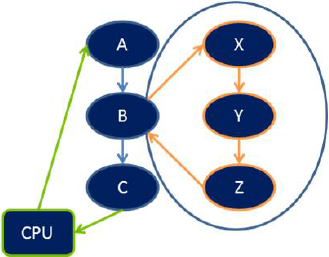
\includegraphics[scale=0.8]{./images/dynamicParallelismSynch}
\end{wrapfigure}
The registers on the GPU are general purpose. Each SM has a number of registers to share
between its cores. If too much register space is used by a kernel, the number of cores per SM that can
be utilized is lowered or local memory\footnote{A portion of device memory
devoted to the storage of local private per thread variables that do not fit
into registers.} can be utilized.
The Geforce GTX 480 has 32.768, 32-bit registers on each of the 15 SMs\footnote{It means 63
32-bit variable per thread for device with cc2.x and 3.0, but that number was
increased to 255 in cc 3.5.} and that memory is 8x faster\footnote{On
Fermi architecture, Volkov http://www.cs.berkeley.edu/~volkov/volkov10-GTC.pdf.
In device with cc 1.x that gap was not so big.} even than the already very
fast shared memory.



\subsection{Dynamic Parallelism}\label{DynamicParallelism}
Cuda 5.0 introduces a new feature,\emph{Dynamic
Parallelism}\cite{dynamicParallelism}\footnote{Only supported by devices with
compute capability 3.5 and higher.} that enable  CUDA kernel to create new work, using the API to launch new kernel,
perform device memory management, or library call (CUBLAS for instance) all
without CPU involvement (see example code \ref{code:dynamicParallelism} at page
\pageref{code:dynamicParallelism}).
This effectively eliminates the superfluous back and forth communication between the GPU and CPU through nested kernel computations.
The launching kernel is called the ``parent'', and the new grid it launches the
``child''.
Child kernels may themselves launch work, creating a nested execution
hierarchy\footnote{To a depth of 24 on Kepler architecture.} and giving the
possibility to easily exploit and port parallel nested algorithms or other
constructs that do not fit a flat, single-level of parallelism.
To be considered complete, a parent kernel all child grids created by its
threads(whichever it is within the kernel) have completed, even if the
programmer does not explicitly synchronize the threads the runtime guarantee
synchronization between parent and all the childs ( see figure
\ref{dynamicparallelismParentChild} and \ref{dynamicParallelismSynch}).
In the example in figure \ref{dynamicParallelismSynch} the kernel C will not be
able to begin execution until kernel Z has completed, because from
the point of view of C, kernels X,Y,Z are seen as part of B.
\begin{figure}
\centering
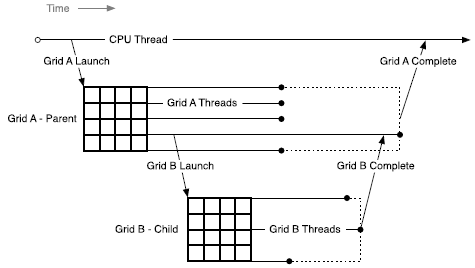
\includegraphics[scale=1.0]{./images/dynamicparallelismParentChild}
\caption{Parent Child Synchronization.}\label{dynamicparallelismParentChild}
\end{figure}
\FloatBarrier 
The same kind of coordination and synchronization holds between X,Y,Z, hence Y
can't begin the execution until X has returned. This allow the program flow can be handled ``on
GPU'' within one single kernel without any memory exchange between GPU and CPU, and also allow hierarchical call to be
written where data from a parent kernel is used to decide how to partition the
next lower level of the hierarchy (see figure
\ref{dynamicparallelismParentChild}) .

Consistency of global memory access is not guarantees between child and parent,
because as usual launches are asynchronous and it means that when a child grid
is invoked it return immediately the control to the parent kernel, and the
parent does not know when child is really executed.
So it can not rely on any assumption about the concurrent execution of the
child. There are just two point in the execution of a child grid when the memory
is fully consistent with the parent:
\begin{itemize}
  \item when a child is invoked.
  \item when the launching thread reaches a synchronization point.
\end{itemize}

Moreover childs and parent grid share the same global and constant memory, but
as kernels, have different and private local registers and shared memory.
It's illegal to use a pointer to local or shared memory as an argument to a
kernel launch.

\begin{figure}
\centering
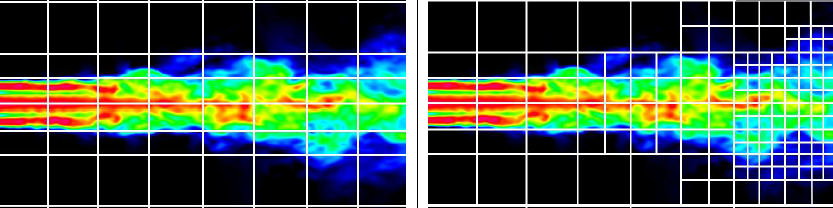
\includegraphics[scale=0.7]{./images/dynamicpParallelismWorkload.png}
\caption{An example of how the parent grid can launch
child grid with dynamic dimension to obtain a better
workload.}\label{dynamicpParallelismWorkload.png}
\end{figure}






\FloatBarrier


\subsection{Performance Guidelines}\label{sect:cudaPerfGuideline}
In this section we discuss some basic, frequently used technique to fully exploit
the computational power of the CUDA platform, but basically they revolve around
these concepts:
\begin{itemize}
  \item Maximize parallel execution to achieve maximum utilization;
 \item  Optimize memory usage to achieve maximum memory throughput;
 \item Optimize instruction usage to achieve maximum instruction throughput.
\end{itemize}


\subsubsection{Maximize Utilization}
At application level the programmer should maximize the device utilization by
using asynchronous function calls and streams\footnote{A CUDA stream is a
sequence of operation that execute in issue order on GPU.}.Different operations
in different streams can run concurrently giving (even if the device support
these kind of operation) better overall performance. At an high level of
abstraction we can think t streams as independent task that could, in theory,
run in parallel without any consequence on each other. At a lower level, the
application should maximize the occupancy. Nvidia provide with its SDK
a spreadsheet that enable the programmer to calculate those metrics\footnote{It can
be found here:
\url{http://developer.download.nvidia.com/compute/cuda/CUDA\_Occupancy_calculator.xls}}
However, maximize the occupancy is not a trivial task, because it can be
influenced by lot of factors and such kernel launch configuration settings,
number of registers utilized by threads or amount of shared memory utilized per block and compute capability.
Another important issue can be represented by the lower utilization of the
functional units. At every instruction issue time, a warp scheduler selects a
warp that is ready to execute its next instruction, if any, and issues the
instruction to the active threads of the warp. The number of clock cycles it
takes for a warp to be ready to execute its next instruction is called the
latency, and full utilization is achieved when all warp schedulers always have
some instruction to issue for some warp at every clock cycle during that latency
period, or in other words, when latency is completely "hidden".
The most common reason a warp is not ready to execute its next instruction is
that the instruction's input operands are not available yet.
For instance if some input operand resides in off-chip memory, the latency is
:400 to 800 clock cycles for devices of  compute capability 1.x and 2.x and
about 200 to 400 clock cycles for devices of compute capability 3.x, that is
much higher than registers's latency which is caused by register dependencies,
i.e. some of them are waiting for some previous instructions to be completed.
Synchronization is another source of latency, because warps waiting at some
synchronizing fence cannot be scheduled.
However is not possible to predeterminate the performance given only a execution
configuration. Experimentation is recommended to find out the best configuration
for the application. Obviously the number of threads per block should be chosen
of multiple of the warps size (i.e. 32) otherwise CUDA automatically pad
the resulting of blocks subdivision warps with \emph{fake} threads, wasting
resources.

\subsubsection{Memory throughput Utilization}
Memory transfer should be avoided, but some of them are
unavoidable especially if they are performed in low bandwidth. For instance
host to/from device bandwidth is much lower than device to device one.
One way to minimize data transfer between the host and the device is to move
more code from the host to the device, even if that means running kernels with
low parallelism computations and try to batch many small transfers into a single
large one, that always perform better.

\subsubsection{Memory throughput Utilization}

Shared memory and caches (i.e., L1/L2 caches available on devices compute
capability 2.x and higher) should be used to minimized memory transfers and
global memory accesses. The typical patter of a program that use shared memory
is :
\begin{itemize}%{labelitemi}{$\Rightarrow$}[leftmargin=1em]
  \renewcommand{\labelitemi}{$\diamondsuit$}
  \item Load data in shared memory. Usually each thread in a block load its
  address.
  \item Synchronize with the other threads so the memory is coherent after its
  population.
  \item Process data in shared memory as much as possible.
  \item Write back to device memory.
\end{itemize}
As explained in section \ref{memoryModel} accesses pattern is important even in
shared memory, so a second phase of optimization is often necessary to organize
accesses in order to enable coalesced access in case of global
memory\footnote{This pattern is more important because the non-optimal global
memory accesses have a higher impact on performance.} or avoid bank conflict
in shared memory.
\subsubsection{Optimize instruction throughput}
Use as much as possible intrinsic\footnote{Less accurate but faster function
directly mapped to fewer with native instruction. They are prefixed with
\emph{\_\_}. The compiler provide an option (\emph{-use-fast\_math}) that
convert automatically each function to an intrinsic one, obviously only those for which an equivalent
intrinsic exist. } function, avoiding function with low throughput and
prefer single precision instead of double precision\footnote{Only when precision
does not affect the end of the result. As we will se in this work, precision is very important.}.
Moreover programmer should be try to minimize thread divergence (see section
\ref{threadDivergence}) in order to not increase the total number of
instruction scheduled for a warp.
There are many other option that can permit a fine-tuning of the application
regarding integer and floating point arithmetics. But those techniques are not
crucial for the performance of the application unless they can give
back a good improvement in some scenarios.\footnote{For a full list of this
operations see CUDA programming guide
:\url{http://docs.nvidia.com/cuda/cuda-c-programming-guide/index.html\#maximize-instruction-throughput}}



\subsubsection{Library usage}
Cuda provide a large yes implemented state of the art functions that span from
linear algebra to AI algorithms\footnote{For the
complete list :https://developer.nvidia.com/technologies/Libraries.}.
Using them instead of writing own kernels one can accelerate the application
development and taking advantage of the performance gain given by the new version of the library due to redesigning of the algorithms or the exploitation of the latest GPU features.
For this work for instance we used Thrust that is a library of parallel
algorithms(sort, scan, transform, reduction etc.) and data structure (see
example code \ref{code:Thrust} at page \pageref{code:Thrust}).



\begin{figure}
\centering
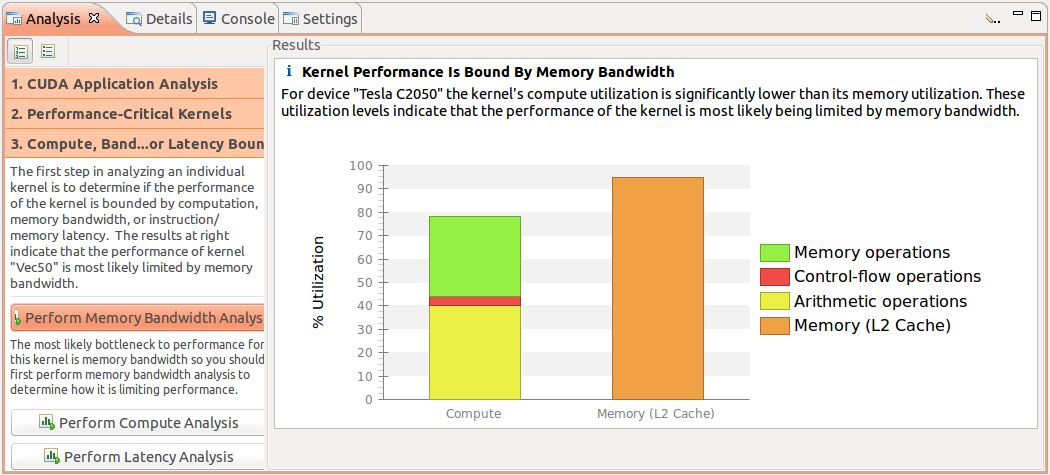
\includegraphics[scale=0.4]{./images/analysis-view.png}
\caption{Example of analysis of a kernel. The profiler gives
lots of metrics that are very useful to perform performance
tuning of the application and to identify bottleneck. In this
case the kernel is very memory bounded.}\label{profiler}
\end{figure}
\subsection{Nvidia Visual Profiler}

The NVIDIA Visual Profiler is a cross-platform performance profiling tool that
delivers developers feedback for optimizing CUDA C/C++ applications, identify
potential performance bottleneck issues and plus it provides optimization suggestions.
These informations are organized in tables that show activity occurring on both
CPU and GPU in a unified time line, including CUDA API calls, memory transfers
and CUDA kernel launches and each information is coupled with many other
statistics and metrics, like timing or occupancy.
This tools has access to the low level metric collected directly from the
hardware and low-level software instrumentation, like power, thermal or clock
situation of the devices.
See figure \ref{profiler} for an example of the kind of suggestions given by
this tools.
